\chapter{Singing Phoneme Recognition} \label{chap:phonerec}
\section{Phoneme recognition using models trained on speech} \label{sec:phonerec_timit}
%timit
%hmm
%dnn 1024x850x1024
% tested: alignment acap
% phonerec acap, dampm/f
%todo: hmm vs dnn??
As a starting point, models for phoneme recognition were trained on speech data, specifically the \textit{TIMIT} corpus. As in many classical ASR approaches, HMMs were selected as a basis and trained using the Hidden Markov Toolkit (HTK)\cite{htk}.\\
Additionally, Deep Neural Networks (DNN) were trained for comparison with models trained on the other data sets. They had three hidden layers of 1024 nodes, 850 nodes, and 1024 nodes again.\\
In both cases, 13 MFCCs were extracted, and deltas and double-deltas were calculated, resulting in a feature vector of dimension 39. As the output, the set of 39 monophones described in section \ref{subsec:tech_systems_phonerec} was used.\\
%output ,mono tri
% results, align, phone
The HMMs were used for aligning text lyrics to audio in some of the following approaches. To verify the quality of such an alignment, this was tested on the part of the \textit{ACAP} singing corpus that has phoneme annotations. On average, the alignment error was $0.16$ seconds. A small manual check suggests that this value may be in the range of the agreement of annotators. A closer inspection of the results also shows that the biggest contribution to this error occur because a few segments were heavily misaligned, whereas most of them are just slightly off.\\
%figure?
The DNN models were trained to perform phoneme recognition. This system was evaluated by first generating phoneme posteriorgrams from the test audio using the DNN models, and then running Viterbi decoding on those to extract phoneme strings. Then, the Phoneme Error Rate and the Weighted Phoneme Error Rate were calculated as described in section \ref{subsec:tech_systems_phonerec}.\\
The results for DNN models trained on \textit{TIMIT} are shown in figure \ref{fig:res_timit}. For validation, the model was tested on the test part of \textit{TIMIT}, resulting in a Phoneme Error Rate of $0.4$ and a Weighted Phoneme Error Rate of $0.3$. Higher values on these corpora can be found in literature, but those systems are usually more sophisticated and include language modeling steps and gender- or speaker-adapted models. In this scenario, those values serve as a validation of the recognition ability of the model on unseen data, and as an upper bound for the other results.\\
On the \textit{ACAP} data set, the phoneme error rate is $1.06$ and the weighted phoneme error rate is $0.8$. Performing the same evaluation on the \textit{DAMP} test data sets generates similar results: A phoneme error rate of $1.26$/$1.29$, and a weighted phoneme error rate of $0.9$. This demonstrates that the performance of models trained on speech leaves room for improvement when used for phoneme recognition in singing. The difference between both singing data sets can be explained by their content: \textit{ACAP} is much smaller, and contains cleaner singing, both considering the recording quality and the singing performance. Songs in this data set were performed by professional singers, whereas the \textit{DAMPTest} sets contain recordings by amateurs who may not always enunciate as clearly. Additionally, the phoneme annotations for the \textit{DAMPTest} sets were generated from the song lyrics; these do not correspond to the actual performed phonemes in all cases.\\
It can be assumed that models trained on better-matching conditions (i.e. singing) would perform much better at this task. The problem with this approach lies in the lack of data sets that can be used for these purposes. In contrast with speech, no large corpora of phonetically annotated singing are available. In the following sections, workarounds for this problem are tested.

\begin{figure*}
	\centering
	\begin{subfigure}[c]{0.45\textwidth}
		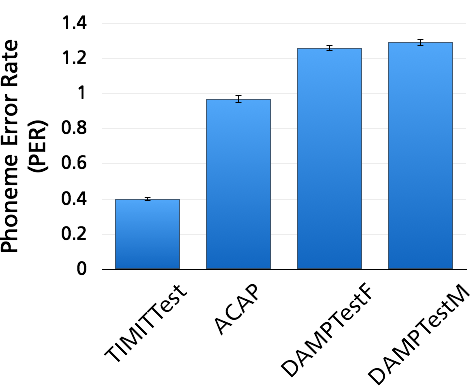
\includegraphics[width=\textwidth]{images/res_timit_per.png}
		\caption{Phoneme error rate}
		
	\end{subfigure}%
	\begin{subfigure}[c]{0.45\textwidth}
		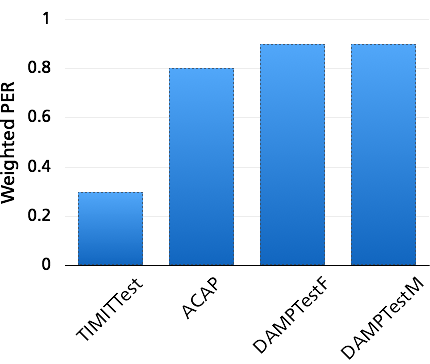
\includegraphics[width=\textwidth]{images/res_timit_wper.png}
		\caption{Weighted phoneme error rate}
	\end{subfigure}
	\caption{Mean phoneme recognition results on the test data sets using acoustic models trained on \textit{TIMIT}.}\label{fig:res_timit}
\end{figure*}



%\section{Phoneme recognition on synthesized singing}
% sinsy; female only
% dnn
%phonerec tested on:
% matched set, acap, dampf
%problem: correct instead of w_per!!
%A first idea to solve the lack of large singing data sets was the use of synthesized singing. For these experiments, the \textit{SYNTH} data set described in section \ref{subsec:data_synth}�was employed. As mentioned, this corpus contains vocal versions of pop songs synthesized with a female voice.\\
%A DNN of the same dimensions as before (1024x850x1024) was trained on the training portion, and then tested on the test portion of \textit{SYNTH}, on the \textit{ACAP} data set, and on the \textit{DAMPTest} sets. The results are displayed in figure \ref{fig:res_synth}.\\

%non-matched: not good (but better than timit??)
% not realistic; just a single voice
% audible accent

\section{Phoneme recognition using models trained on ``songified" speech}
% time stretch, pitch shift
% variants
% dnn vs dbn??
% phonerec tested on: timit, acap
% todo: test on damp

When there is a scarcity of suitable training data, attempts are often made to generate such data artificially from existing data for other conditions. For example, this is often done when models for noisy speech are required \cite{ntimit}\cite{aurora}. Inspired by this, one idea was making existing speech data sets more ``song-like'' and use these modified datasets to train models for phoneme recognition in singing. The \textit{TIMIT} corpus was once again used as a basis for this.\\

An overview of the approach is shown in figure \ref{fig:process_songify}. Five variants of the training part  \textit{TIMIT} were generated first. MFCC features were then extracted from these new datasets and used to train models.\\
Similarly, MFCCs are extracted from the \textit{TIMIT} Test set and from the \textit{ACAP} data set. The previously trained models are used to recognize phonemes on these test datasets. Viterbi decoding can then be used to generate phoneme sequences. Finally, the results are evaluated.

%TODO: check
\begin{figure*}
 \begin{center}
                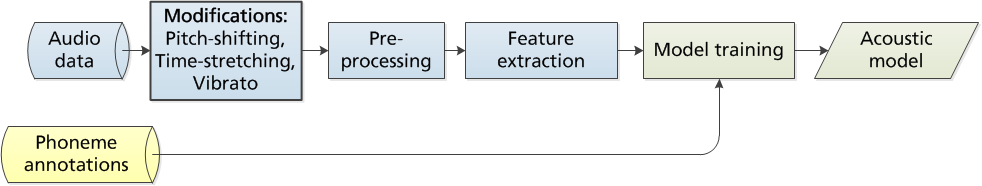
\includegraphics[width=1\textwidth]{images/process_training_phones_songify.png}
                \caption{Overview of the ``songified'' phoneme recognition training process.}
                \label{fig:process_songify}
                 \end{center}
 \end{figure*}
In order to make the training data more ``song-like'', several variants of this dataset were developed. Table \ref{tab:timit_variants} shows an overview over the five datasets generated from \textit{TIMIT} using three modifications. Dataset $N$ is the original \textit{TIMIT} training set. For dataset $P$, four of the eight blocks of \textit{TIMIT} were pitch-shifted. For dataset $T$, five blocks were time-stretched and vibrato was applied to two of them. In dataset $TP$, the same is done, except with additional pitch-shifting. Finally, dataset $M$ contains a mix of these modified blocks.\\
In detail, the modifications were performed in the following way:

\begin{description}
 \item[Time stretching] For time stretching, the phase vocoder from \cite{ellis_pvoc}, which is an implementation of the Flanagan/Dolson phase vocoder \cite{flanagan}\cite{dolson}, was used. This algorithm works by first performing a Short-Time Fourier Transform (STFT) on the signal and then resampling the frames to a different duration and performing the inverse Fourier transform.\\
 As demonstrated in section \ref{sec:sota_speechtosinging}, time variations in singing are mainly performed on vowels and are often much longer than in speech. Therefore, the \textit{TIMIT} annotations were used to only pick out the vowel segments from the utterances. They were modified randomly to a duration between $5$ and $100$ times the original duration and then re-inserted into the utterance. This effectively leads to more vowel frames in the training data, but since there is already a large amount of instances for each phoneme in the original training data, the effects of this imbalance should be negligible. 
 \item[Pitch shifting] To pitch-shift the signal, code from the freely available Matlab tool \textit{AutoTune Toy}\cite{autotunetoy}, which also implements a phase vocoder, was used. In this case, the fundamental frequency is first detected automatically. The signal is then stretched or expanded to obtain the new pitch and interpolated to retain the original duration.\\
 Using the \textit{TIMIT} annotations, utterances were split up into individual words, and then a pitch-shifted version of each word was generated and the results were concatenated. Pitches are randomly selected from a range between $60\%$ and $120\%$ of the original pitch.
 \item[Vibrato] The code for vibrato generation was also taken from \textit{AutoTune Toy}. It functions by generating a sine curve and using this as the trajectory for the pitch shifting algorithm mentioned above. A sine of amplitude $0.2$ and frequency 6Hz was used.\\
 In singing, vibrato is commonly done on long sounds, which are usually vowels. Since spoken vowels are usually very short, vibrato cannot be perceived on them very well. Therefore, vibrato was only added when time stretching was also applied. Vibrato was then added to the extracted and stretched vowels.
\end{description}



\begin{table}
 \begin{center}
  \begin{tabular}{|c||c|c|c|c|c|}
  \hline
   & \textbf{N} & \textbf{P} &\textbf{T} &\textbf{TP} &\textbf{M} \\
  \hline
  DR1 & N & N & N & N & N  \\
  DR2 & N & N & N & N & N \\
  DR3 & N & N & N & N & P\\
  DR4 & N & N & T & TP & TV \\
  DR5 & N & P & T & TP & TPV \\
  DR6 & N & P & T & TP & TV \\
  DR7 & N & P & TV & TPV & P \\
  DR8 & N & P & TV & TPV & TPV \\
  \hline
 \end{tabular}
\end{center}
 \caption{The five TIMIT variants that were used for training (rows are TIMIT blocks, columns are the five datasets).
  Symbols: N - Unmodified; P - Pitch-shifted; T - Time-stretched; V - Vibrato}
 \label{tab:timit_variants}
\end{table}


\begin{figure*}
	\centering
	\begin{subfigure}[c]{0.5\textwidth}
		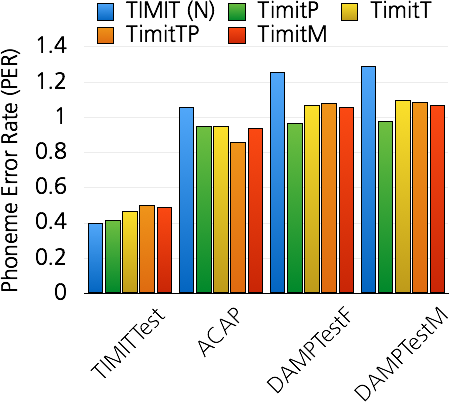
\includegraphics[width=\textwidth]{images/res_songify_per.png}
		\caption{Phoneme error rate}
		
	\end{subfigure}%
	\begin{subfigure}[c]{0.5\textwidth}
		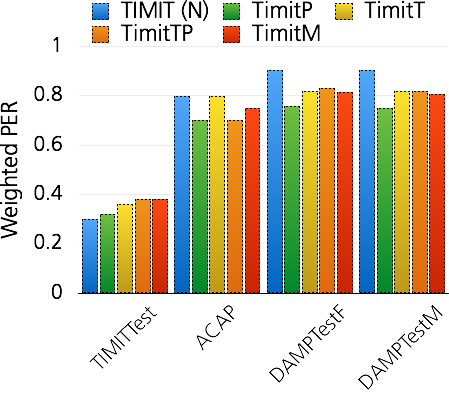
\includegraphics[width=\textwidth]{images/res_songify_wper.png}
		\caption{Weighted phoneme error rate}
	\end{subfigure}
	\caption{Mean phoneme recognition results on the test data sets using acoustic models trained on \textit{TIMIT} and augmented versions thereof.}\label{fig:res_songify}
\end{figure*}
The approach was tested on the various test data sets - namely, the test part of \textit{TIMIT}, the \textit{TIMIT} data set, and the two test sets chosen from the \textit{DAMP} data set. Figure \ref{fig:res_songify} shows the results for the DNN models. As it demonstrates, results for singing are generally worse than for speech. The base result for singing is a Weighted Phoneme Error Rate of $0.8$ for \textit{ACAP}, and of $0.9$ for both \textit{DAMPTestF} and \textit{DAMPTestM} (model trained on the original TIMIT dataset). When comparing the models trained on the various \textit{TIMIT} modifications, an improvement is observed for all variants. In contrast, none of the modifications improved the result on the speech data at all. The base result here $0.3$. (see previous section). This makes sense since all of the modifications make the training data less similar to the test data set.\\
On singing, the Weighted Phoneme Error rate falls by $0.1$ to $0.15$ when using models trained on the pitch-shifted data set (\textit{TimitP}), and by up to $0.08$ when using the time-stretched training data (\textit{TimitT}). The improvements for the corpora with both improvements lie in between. Vibrato does not appear to have a strong influence on the result. The higher error rates for \textit{DAMPTest} can, again, be explained with the fact that this data set has more variation in audio and singing quality.\\
%pitch shift: stronger, actual new feature values instead of just more; more realistic than long vowels because of shaping??
Pitch shifting might have a stronger effect on the recognition result because it is a stronger modification in the sense that it generates actual new feature values. In contrast, time stretching mostly generates new frames with values similar to the ones in the original data set (and only in between those). Additionally, pitch shifting may introduce more variety that is closer to sung sounds because singers do not usually shape long vowels just by stretching out their short versions.\\
Nevertheless, it is interesting to see that both pitch shifting and time stretching improve the result for sung phoneme recognition. This indicates that more variety in the training data is a step in the right direction. However, there is still a lot of room for improvement.





\section{Phoneme recognition using models trained on a-capella singing} \label{sec:phonerec_acap}
%how created?
% dnn
%phonerec tested on:
% acap, dampf/m
%alignment tested on acap; also: hmms!!
In this section, the most salient tested approach for phoneme recognition in singing is presented. For this method, acoustic models were trained on actual singing recordings. A large set of such recordings was already available from the \textit{DAMP} corpus, but no annotations were included with them. Such annotations were generated automatically from text lyrics available on the internet. In the following subsections, this process is described in detail, some variants are tested, and experiments with these new models are presented. 

\subsection{Corpus construction}\label{subsec:phonerec_corpus}



\begin{figure*}
 \begin{center}
                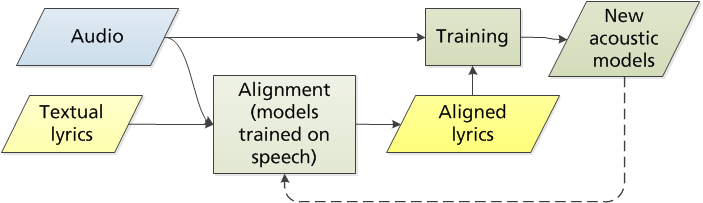
\includegraphics[width=.8\textwidth]{images/process_bootstrap.png}
                \caption{An overview of the alignment process. The dotted line represents the optional bootstrapping.}
                \label{fig:damp_alignment_process}
                 \end{center}
 \end{figure*}
 
As mentioned above, no lyrics annotations are available for the \textit{DAMP} data set, but the textual lyrics can be obtained from the \textit{Smule Sing!} website\footnote{\url{http://www.smule.com/songs}}.  All of them were English-language songs. These lyrics were mapped to their phonetic content using the CMU Pronouncing Dictionary\footnote{\url{http://www.speech.cs.cmu.edu/cgi-bin/cmudict}} with some manual additions of unusual words. As with the other data sets, this dictionary has a phoneme set of 39 phonemes (also see appendix \ref{app:phonemes}).\\
An automatic alignment of these lyrics to the \textit{DAMP} audio was then performed using the HMM acoustic models trained on \textit{TIMIT} (see section \ref{sec:phonerec_timit}). Viterbi alignment was performed on the word and phoneme levels using the HTK framework, using MFCCs and their deltas and double-deltas as features. This is the same principle of so-called ``Forced Alignment" that is commonly used in Automatic Speech Recognition \cite{book:jurafsky} (although it is usually done on shorter utterances). \\
Several different alignment strategies were carried out:
\begin{description}

\item[One state vs. three states per phoneme] Versions with one state per phoneme and three states per phoneme (so-called ``senones'', modeling the start, middle, and end phases) were tested. Since \textit{TIMIT} only contains single-phoneme annotations, this was done by first splitting the phoneme time frames evenly through three, and then re-training the \textit{TIMIT} acoustic model and re-aligning the data set (with the assumption that the transitions between the three states would be ``pulled'' to the correct times).  
\item[One-pass alignment vs. Bootstrapping] On top of a one-pass alignment using the Viterbi algorithm, bootstrapping the acoustic models to improve the alignment was also. To clarify: The alignment was first performed on the \textit{DAMP} data sets using the \textit{TIMIT} models described above, then acoustic models were trained on the resulting phoneme annotations. Then, those models were used to re-align the \textit{DAMP} data, which was again used to train another model. This was done over three iterations.\\
A modified version of the alignment algorithm was used for doing alignment with the models trained on the \textit{DAMP} data sets. This approach is based on doing Dynamic Time Warping on the generated phoneme posteriorgrams without punishing very long states. This is similar to the approach described in \ref{sec:ret_post}.
\end{description}
A graphical overview of the alignment process is given in figure \ref{fig:damp_alignment_process}.\\
Of course, errors cannot be avoided when doing automatic forced alignment. All in all, there were now four combinations of these strategies, which were compared. The next section describes how this alignment procedure was validated and what strategies performed best.\\
Since there is usually a large number of recordings of the same song, an approach using this information to improve the alignment results was also considered, e.g. by averaging time stamps over the alignments of several recordings. This was not done in this work because recordings tend to have different offsets from the beginning (i.e. silence in the beginning), and the singers also do not necessarily pronounce phonemes at the same time. This might be an avenue for future research, though.

%\subsection{Validation}\label{sec:validation}
%Validating the phoneme annotations created in this way is not trivial since there is no ground truth to base them on. Therefore, a two-pronged approach was employed: The same alignment algorithm was first tested on the small, manually annotated \textit{ACAP} data set. Second, new acoustic models were trained on the newly generated training data sets. Then, phoneme recognition was performed on the test data sets, and the results were compared to the expected phoneme strings (which are known from the matching lyrics).

\subsection{Alignment validation}
The alignment approach that was used to create the new \textit{DAMP}-based data sets was first tested on the \textit{ACAP} data set. To recap: This approach employs models trained on the \textit{TIMIT} speech corpus, which are used for Viterbi alignment of the known phonemes to the singing. The result of this is then compared to the manual annotations by calculating the difference between each expected and predicted phoneme transition. As mentioned in \ref{sec:phonerec_timit} and shown in figure \ref{fig:res_alignment}, the mean alignment error for this first approach is $0.16$ seconds for the three-state case, and $0.17$ for single phoneme states.\\

%TODO: other figure
\begin{figure}
	\begin{center}
		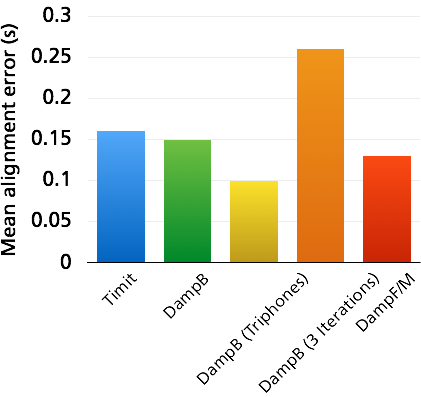
\includegraphics[width=.8\textwidth]{images/res_alignment.png}
		\caption{Mean alignment error in seconds on the \textit{ACAP} data set. \textit{TIMIT} shows the result for the same models used for aligning the new \textit{DAMP}-based data sets.}
		\label{fig:res_alignment}
	\end{center}
\end{figure}


Various models trained on the new \textit{DampB}, \textit{DampF}, and \textit{DampM} training data sets were then tested for the same task. The results are also shown in figure \ref{fig:res_alignment}.\\
Models trained on the monophonic alignments of \textit{DampB} perform slightly better at this task with mean errors of $0.15$ seconds. For the gender-specific models, the error was only calculated for the songs of the matching gender in \textit{ACAP}, resulting in the same average value. Since the gender-specific models do not produce better results, the other experiments were conducted on the mixed training set only. The three-state version of \textit{DampB} performs even better at alignment, with a mean error of $0.1$. This might happen because dedicatedly training the model for the start and end parts of phonemes might make the alignment approach more accurate at finding start and end points.\\
Finally, a model trained on \textit{DampB} over three iterations was also tested for alignment. This model performs much worse at this task with a mean alignment error of $0.26$. This might happen because errors in the original alignment of the phonemes may become amplified over these iterations. The effect is not as pronounced for the three-state version, but it is still present.


\begin{figure*}
	\centering
	\begin{subfigure}[c]{0.5\textwidth}
		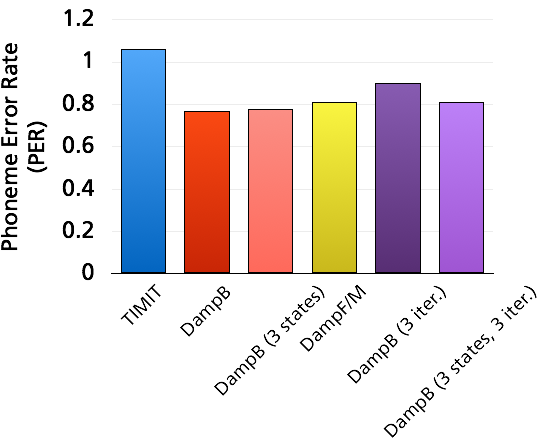
\includegraphics[width=\textwidth]{images/res_phonerec_acap.png}
		\caption{Phoneme error rate}
		
	\end{subfigure}%
	\begin{subfigure}[c]{0.5\textwidth}
		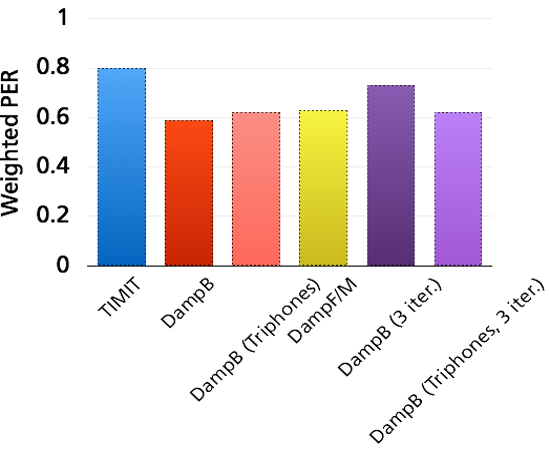
\includegraphics[width=\textwidth]{images/res_phonerec_acap_w.png}
		\caption{Weighted phoneme error rate}
	\end{subfigure}
	\caption{Mean phoneme recognition results on the \textit{ACAP} data set using acoustic models trained on \textit{Timit} and the new \textit{DAMP}-based data sets.}\label{fig:res_phonerec_acap}
\end{figure*}

\begin{figure*}
	\centering
	\begin{subfigure}[c]{0.5\textwidth}
		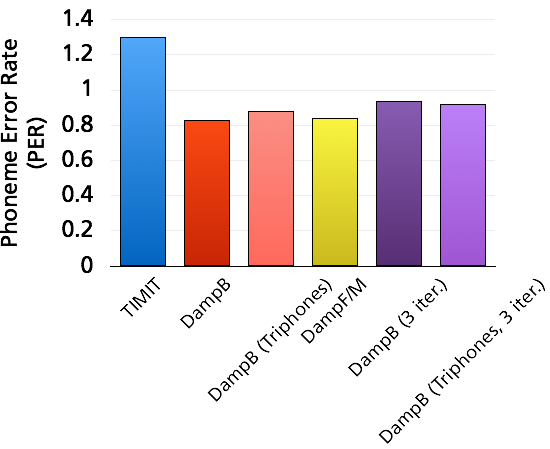
\includegraphics[width=\textwidth]{images/res_phonerec.png}
		\caption{Phoneme error rate}
		
	\end{subfigure}%
	\begin{subfigure}[c]{0.5\textwidth}
		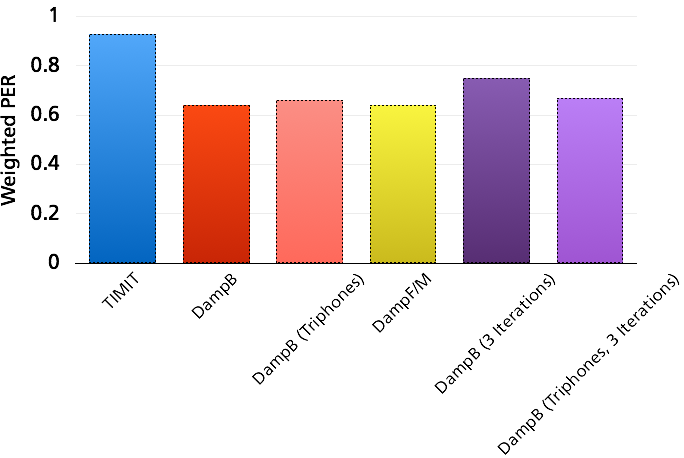
\includegraphics[width=\textwidth]{images/res_phonerec_w.png}
		\caption{Weighted phoneme error rate}
	\end{subfigure}
	\caption{Mean phoneme recognition results on the \textit{DampTest} data sets using acoustic models trained on \textit{TIMIT} and the new \textit{DAMP}-based data sets.}\label{fig:res_phonerec}
\end{figure*}


\begin{figure*}
	\centering
	\begin{subfigure}[c]{0.5\textwidth}
		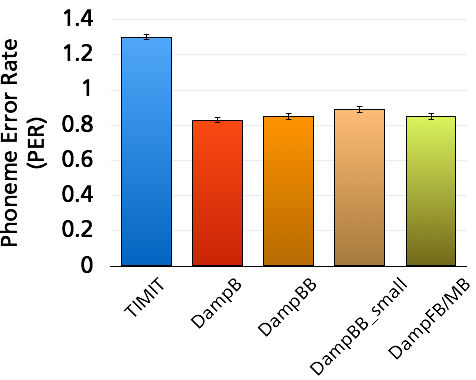
\includegraphics[width=\textwidth]{images/res_phonerec_sizes.png}
		\caption{Phoneme error rate}
		
	\end{subfigure}%
	\begin{subfigure}[c]{0.5\textwidth}
		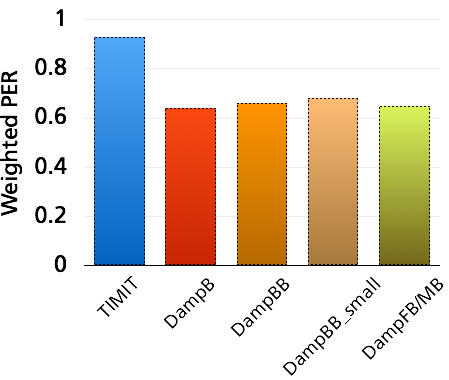
\includegraphics[width=\textwidth]{images/res_phonerec_sizes_w.png}
		\caption{Weighted phoneme error rate}
	\end{subfigure}
	\caption{Mean phoneme recognition results on the \textit{DampTest} data sets using acoustic models trained on \textit{TIMIT} and the new \textit{DAMP}-based data sets.}\label{fig:res_phonerec_sizes}
\end{figure*}

\subsection{Phoneme recognition}
After validating the alignment strategy, phoneme recognition experiments were performed on both the \textit{ACAP} and the \textit{DampTest} corpora. This was possible even though there are no manual annotations for the \textit{DampTest} sets because the expected phonemes are available from the textual lyrics. Again, the phoneme error rate and the weighted phoneme error rate were used as evaluation measures (see \ref{subsec:tech_systems_phonerec}).\\
The results for \textit{ACAP} are shown in figure \ref{fig:res_phonerec_acap}. In general, models trained on \textit{DampB} performed much better at phoneme recognition than those trained on \textit{TIMIT}. Compared to these speech-based models, the phoneme error rate falls from $1.06$ to $0.77$, while the weighted phoneme error rate falls from $0.8$ to $0.59$. As can be seen from both evaluation measures, using alignments with three states per phoneme instead of single states does not improve the results in this case, contrasting with the better alignment results. This might happen because more classes cause more confusion in the model, even though the three-state results were downmapped to single phonemes for calculating the evaluation measures. Additionally, the temporal pronunciation phases may just be too variable in singing, as opposed to speech. As in the alignment results, using gender-specific models does not provide an advantage over a mixed model. (Results for the gender-specific models were only evaluated on songs of the matching gender).\\
As already seen in the alignment validation results, training models on \textit{DampB} over three iterations actually degrades the result. Again, this might happens because phoneme alignment errors become amplified in this way. Interestingly, the effect is not as strong for the three-state models, perhaps because the three classes per phoneme help to alleviate each other's errors.\\

The results for the same procedure on the \textit{DampTest} sets are shown in figure \ref{fig:res_phonerec}. Results over \textit{DampTestF} and \textit{DampTestM} were averaged.
The same general trend can be observed for these results: The phoneme error rate falls from $1.3$ to $0.83$ when compared to models trained on \textit{TIMIT}, with the weighted phoneme error rate decreasing from $0.93$ to $0.64$. Using three states per phoneme does not contribute to the result, and neither does the three-iteration bootstrapping process for training acoustic models. As in the \textit{ACAP} results, not even the gender-specific models improve the result. This effect might occur because the range of pitch and expressions is much wider in singing than in speech, and therefore gender-specific models may not actually learn as much added helpful information. Other experiments indicated that gender-specific models also do not improve the results when using three states or three alignment iterations as with the mixed-gender training data.\\

Going forward, single-state models trained on mixed-gender data (i.e. \textit{DampB}) appear to be the best and simplest solution. To gain insight into the role of the composition of the training data set, more experiments were conducted with the variants of \textit{DampB} described in section \ref{sec:data_damp}. The results are shown in figure \ref{fig:res_phonerec_sizes}.\\

When using the smaller, more balanced version of \textit{DampB} (\textit{DampBB}), the results become somewhat worse, but not much, with a phoneme error rate of $0.85$, and a weighted phoneme error rate of $0.66$. This is particularly interesting because this data set is only 4\% the size of the bigger one and training is therefore much faster. With the smallest data set which is only half the size of \textit{DampBB}, the change is similar: The Phoneme Error Rate rises to $0.89$, the Weighted Phoneme Error Rate to $0.68$. Since this data set has roughly the same amount of phonemes as \textit{TIMIT}, this proves that the improvement is actually caused by the acoustic properties of the training data, rather than just the larger amount of data. (Of course, this factor also contributes). The reduced versions of \textit{DampF} and \textit{DampM} were tested as well, but once again, they do not provide an improvement over the mixed gender model.\\


\subsection{Error sources}\label{subsec:error_sources}
Of course, with an automatic alignment algorithm like this, errors cannot be avoided. To acquire a clearer picture of the reasons for the various misalignments, the audio data where they occurred was analyzed more closely. Some sources of error repeatedly stuck out:
%\begin{compactdesc}
\begin{description}
 \item[Unclear enunciation]{Some singers pronounced words very unclearly, often focusing more on musical performance than on the lyrics.}
 \item[Accents]{Some singers sung with an accent, either their natural one or imitating the one used by the original singer of the song.}
 \item[Young children's voices]{Some recordings were performed by young children.}
 \item[Background music]{Some singers had the original song with the original singing running in the background.}
 \item[Speaking in breaks]{Some singers spoke in the musical breaks.}
 \item[Problems in audio quality]{Some recordings had qualitative problems, especially loudness clipping.}
%\end{compactdesc}
\end{description}
For most of these issues, more robust phoneme recognizers would be helpful. For others, the algorithm could be adapted to be robust to extraneous recognized phonemes (particularly for the speaking problem). If possible, a thorough manual check of the data would be very helpful as well.



\section{Conclusion}
% timit starting point
% songified somewhat better (what?)
% best: actual singing
% problem: no annotations
% solution: get text lyrics, align with timit models; alignment verified on acap
% best results on speech (easiest)
% acap better than damp test sets
% because: better enunciation, homogenous recording quality, fewer annotation errors (!!)
% gender-specific not helpful
%triphones sometimes help, sometimes not
% iterating amplifies errors
% decimating training data still produces good models
% overtraining???
% error sources
In this chapter, new approaches for phoneme recognition in singing were described. As a starting point, DNN models were trained on the \textit{TIMIT} speech corpus. For verification, these models were evaluated on the test section of \textit{TIMIT}, resulting in a Phoneme Error Rate of $0.4$ and a Weighted Phoneme Error Rate of $0.3$. The results on the \textit{ACAP}�singing data set were much worse: A Phoneme Error Rate of $1.06$ and a Weighted Phoneme Error Rate of $0.8$, demonstrating the difficulty of phoneme recognition in singing as opposed to speech. Similarly, the Phoneme Error Rate was $1.28$ on the \textit{DampTest} data sets, with a Weighted Phoneme Error Rate of $0.9$. Generally, results on the \textit{DampTest} sets are worse than on the \textit{ACAP} test set, which presumably happens because the \textit{DampTest} sets are performed by amateurs, whose enunciation is not as clear as that of the professional singers in the \textit{ACAP} set and who may not always sing the correct lyrics, because the recording quality varies much more, and because the annotations may contain errors due to the automatic phoneme alignment (as opposed to the more realiable manual annotations of \textit{ACAP}).\\

In order to make the models better adapted to singing, acoustic modifications were performed on the \textit{TIMIT} training data - namely, pitch shifting and time stretching. This increases the Phoneme Error Rate on speech test data (\textit{TIMITTest}, but improves them on sung data. Pitch shifting appears to have a stronger effect than time stretching, which might happen because this modification results in actual changed feature data, whereas time stretching mainly produces more frames with feature values similar or in between the existing ones. On the \textit{ACAP} test data, the lowest Phoneme Error Rate is $0.95$, and the lowest Weighted Phoneme Error Rate is $0.7$ (with the pitch-shifted models). On \textit{DampTest}, those values are decreased to $0.98$ and $0.76$ respectively.\\

The best-adapted models for recognizing phonemes in singing should be those trained on actual singing data. Unfortunately, there are no big, annotated singing data sets like those for speech. For this reason, the \textit{DAMP} data set, which contains thousands of recordings of unaccompanied amateur singing, was selected, and the text lyrics were obtained from the internet. Then, various strategies for aligning the phonetic content of these lyrics to the audio were tested. In the simplest algorithm, HMM models trained on \textit{TIMIT} were used for Viterbi alignment. This also turned out to be one of the most effective algorithms for the alignment process necessary for constructing this new singing data set.\\

The resulting annotations, together with the singing audio data, were then used to train new DNN models for phoneme recognition. Using 6000 of these recordings of singers of both genders, the Phoneme Error Rate was lowered to $0.77$ on the \textit{ACAP} test set, and the Weighted Phoneme Error Rate was lowered to $0.59$. On the \textit{DampTest} sets, those values decreased to $0.83$ and $0.64$ respectively. Neither employing three states per phoneme instead of a single state nor training gender-specific models provided additional advantages. Iterating the alignment process decreased the result, possibly because errors in the original alignment become amplified over these iterations.\\

The influence of training set size was also investigated on the \textit{DampTest} data. Using a phonetically balanced subset of \textit{DAMP} that was just $4\%$ of the size of the originally selected training set worsened the result by only 2 percent points (both in Phoneme Error Rate and Weighted Phoneme Error Rate). Using an even smaller data set that is roughly the size of \textit{TIMIT} increased the Phoneme Error Rate only by a further 4 percent points (and the Weighted Phoneme Error Rate by 2), thereby proving that the better recognition results are caused by the sung content rather than just the size of the training data.\\
%OVERTRAINING???

%!!!
A manual error analysis was performed on cases where the phoneme recognition failed. Errors are frequently caused by linguistically or acoustically difficult segments in the test data, such as accents, children's voices, background music, or additional speaking.\\

Comparing these results to the state of the art is difficult because of the different testing data used. Considering raw numbers, it can be assumed that the best results are in the range of the best state of the art results, for example those by Mesaros et al. \cite{Mesaros2011} (see section \ref{sec:sota_phonerec}). In contrast to these approaches, no involved post-processing is employed. In the future, integrating such steps as singer adaptation and language modeling would in all probability serve to improve the approach even more.\\
Another option that has not been tested yet is the use of triphones (i.e. training tied models for phonemes with context dependency on their predecessors and successors). This approach is frequently used in ASR.



